\documentclass[10pt,a4paper]{article}

% ── Packages ──
\usepackage[utf8]{inputenc}
\usepackage[T1]{fontenc}
\usepackage{lmodern}
\usepackage[margin=2.5cm]{geometry}
\usepackage{graphicx}
\usepackage{booktabs}
\usepackage{amsmath}
\usepackage{amssymb}
\usepackage{hyperref}
\usepackage{xcolor}
\usepackage{authblk}
\usepackage{multirow}
\usepackage{caption}
\usepackage{subcaption}
\usepackage{lineno}
\usepackage{setspace}
\usepackage{natbib}

\bibliographystyle{unsrtnat}

\hypersetup{
    colorlinks=true,
    linkcolor=blue!60!black,
    citecolor=blue!60!black,
    urlcolor=blue!60!black,
}

% ── Line numbers ──
\linenumbers
\onehalfspacing

% ── Title ──
\title{\textbf{DeepMiRT: miRNA target prediction using RNA foundation models and cross-attention}}

\author{Zicheng Liu}
\date{}

\begin{document}

\maketitle

% ============================================================
% Abstract
% ============================================================
\begin{abstract}
MicroRNAs (miRNAs) are $\sim$22-nucleotide non-coding RNAs that post-transcriptionally regulate gene expression by guiding Argonaute proteins to complementary sites in target mRNAs. Accurate computational prediction of miRNA--target interactions is essential for understanding regulatory networks, yet existing tools rely on hand-crafted thermodynamic features or shallow sequence models that struggle to capture the full complexity of target recognition. Here we present DeepMiRT, a deep learning framework that leverages RNA-FM, a 12-layer Transformer foundation model pre-trained on 23 million non-coding RNA sequences, as a shared encoder for both miRNA and target sequences. A two-layer, eight-head cross-attention mechanism allows the target representation to query the miRNA at every position, learning complementarity patterns beyond canonical seed matching. We train on 8.1 million miRNA--target pairs compiled from multiple species---predominantly human and mouse, with smaller contributions from \textit{C.\ elegans}, \textit{Drosophila}, and other organisms---with the RNA-FM backbone frozen, optimizing only the cross-attention and classification head ($\sim$4M trainable parameters out of 103M total). On a held-out test set of 813{,}329 samples, DeepMiRT achieves an AUROC of 0.9606 [95\% CI: 0.9602--0.9610] and AUPRC of 0.9669 [0.9666--0.9672], outperforming the second-best method by 7.5 percentage points. When re-evaluated on miRBench standardized test datasets, DeepMiRT ranks first among 12 methods on both eCLIP datasets in both AUROC (0.7511 and 0.7524) and average precision (APS: 0.7850 and 0.7947). The model exhibits excellent probability calibration (expected calibration error = 0.0064) and generalizes to miRNAs completely unseen during training (AUROC = 0.943). DeepMiRT is available as an open-source Python package (\texttt{pip install deepmirt}), with pre-trained weights hosted on Hugging Face Hub and an interactive web demo for immediate use.
\end{abstract}

\vspace{0.5em}
\noindent\textbf{Keywords:} miRNA target prediction, RNA foundation model, cross-attention, deep learning, transfer learning

\vspace{1em}

% ============================================================
% 1. Introduction
% ============================================================
\section{Introduction}

MicroRNAs (miRNAs) are endogenous non-coding RNAs of approximately 22 nucleotides that serve as master post-transcriptional regulators across metazoans~\citep{bartel2009, bartel2018}. By guiding the RNA-induced silencing complex (RISC) to complementary sites---typically in the 3$'$ untranslated region (UTR) of messenger RNAs---miRNAs direct translational repression or mRNA degradation. A single miRNA can regulate hundreds of target transcripts, and more than 60\% of human protein-coding genes are estimated to be under miRNA control~\citep{bartel2018}. In insects, miRNAs play critical roles in development, metamorphosis, immunity, and adaptation to environmental stress~\citep{asgari2013insect, lucas2013insect}. With rapid advances in insect genome sequencing, accurate computational prediction of miRNA--target interactions has become essential for functional annotation in non-model arthropod species, yet the existing tool ecosystem remains heavily biased toward vertebrate biology.

Computational target prediction has a long history. First-generation rule-based methods such as seed matching~\citep{bartel2009}, miRanda~\citep{enright2003miranda}, and RNAhybrid~\citep{rehmsmeier2004rnahybrid} exploit thermodynamic stability of the miRNA--target duplex and complementarity of the seed region---the 6--8 nucleotide stretch at the miRNA 5$'$ end that is most critical for target recognition. These approaches are fast and interpretable, but they produce high false-positive rates because thermodynamic stability alone does not determine functional targeting. Second-generation machine-learning approaches, exemplified by TargetScan~\citep{agarwal2015targetscan, mcgeary2019targetscan}, incorporate evolutionary conservation, local AU content, and target site accessibility, achieving better specificity at the cost of requiring vertebrate-specific conservation data. Third-generation deep learning methods such as TargetNet~\citep{min2022targetnet}, CnnMirTarget~\citep{zheng2020cnnmirtarget}, miRBind~\citep{klimentova2022mirbind}, miRNA\_CNN~\citep{hejret2023chimeric}, and the InteractionAwareModel~\citep{yang2024interaction} train convolutional or attention-based neural networks directly on miRNA--target sequence pairs, learning features end-to-end without manual engineering.

Despite progress, existing methods face three key limitations that motivate our work. First, most tools are trained exclusively on human or \textit{C.\ elegans} data and have limited transferability to insects, where miRNA--target co-evolution across $\sim$400 million years has produced divergent binding patterns, different 3$'$UTR architectures, and species-specific miRNA families with no direct mammalian orthologs. Furthermore, conservation-based features---central to TargetScan's predictive power---are largely unavailable for most insect lineages due to the lack of deeply aligned multi-species genomes. Second, each existing deep learning method learns sequence features entirely from scratch, using only the relatively small corpus of experimentally validated miRNA--target interactions (typically tens of thousands of positive examples). This approach ignores the rich structural and evolutionary information encoded in the much larger universe of RNA sequences across the tree of life---information that could provide a strong inductive bias for learning binding patterns. Third, most methods rely heavily on seed complementarity as the primary signal, and consequently struggle to detect non-canonical binding sites. CLASH data suggest that around 60\% of miRNA seed interactions involve noncanonical pairing (bulges or mismatches), and 18\% of interactions are mediated by the miRNA 3$'$ end with little 5$'$ seed contact~\citep{helwak2013clash}. A method that could learn richer sequence representations might better capture these diverse binding modes.

Pre-trained foundation models---large neural networks trained on massive unlabeled datasets via self-supervised objectives---have transformed multiple domains of computational biology. In protein science, ESM-2~\citep{lin2023esm} demonstrated that language models trained on protein sequences capture evolutionary and structural information sufficient for atomic-level structure prediction. In natural language processing, BERT~\citep{devlin2019bert} showed that masked language modeling on large text corpora produces representations that transfer to diverse downstream tasks with minimal task-specific training. In the RNA domain, RNA-FM~\citep{chen2022rnafm} is a 12-layer Transformer model with 640-dimensional hidden states, pre-trained on 23 million non-coding RNA sequences from RNAcentral via masked nucleotide prediction. RNA-FM has demonstrated strong zero-shot and fine-tuning performance on downstream tasks including secondary structure prediction (F1 $>$ 0.96 on bpRNA), functional classification, and distance map estimation, suggesting that it learns meaningful representations of RNA sequence and structure. More recently, RiNALMo~\citep{rinalmo2025} extended this approach to 36 million sequences with larger architecture, further validating the foundation model paradigm for RNA. Despite this progress, the potential of RNA foundation models for miRNA--target interaction prediction---a pairwise classification task requiring modeling of inter-sequence complementarity---remains unexplored.

Here, we present DeepMiRT (\textbf{Deep} learning for \textbf{Mi}RNA \textbf{R}NA-FM \textbf{T}arget prediction), a framework that repurposes RNA-FM as a shared encoder for both miRNA and target sequences, connected by a cross-attention module~\citep{vaswani2017attention} that captures interaction-level features without requiring manual feature engineering. The shared encoder ensures that miRNA and target representations lie in a common embedding space learned from 23 million RNA sequences, while cross-attention explicitly models position-wise complementarity---allowing the model to jointly assess seed pairing, 3$'$ compensatory binding, and other positional signals. By training only the cross-attention and classification head (4M out of 103M parameters) while keeping the RNA-FM backbone frozen, DeepMiRT achieves state-of-the-art performance on eCLIP-based benchmarks while maintaining excellent probability calibration and robust generalization to miRNA sequences entirely unseen during training. Our contributions are: (1) the first application of pre-trained RNA foundation models to miRNA target prediction; (2) a cross-attention architecture that explicitly models miRNA--target interaction at every position; (3) comprehensive benchmarking against 11 published methods on standardized datasets; and (4) an open-source Python package with pre-trained weights and a web demo, released to facilitate adoption by the broader genomics community.

% ============================================================
% 2. Methods
% ============================================================
\section{Methods}

\subsection{Architecture}

DeepMiRT consists of three components (Figure~\ref{fig:architecture}): (i) a shared RNA-FM encoder, (ii) a cross-attention interaction module, and (iii) a multi-layer perceptron (MLP) classification head.

\paragraph{Shared RNA-FM encoder.} Both the miRNA sequence ($\sim$18--25 nt) and the target site fragment (40 nt) are tokenized using the RNA-FM vocabulary and independently processed by the same RNA-FM encoder~\citep{chen2022rnafm}. RNA-FM is a 12-layer Transformer with 20 attention heads per layer and 640-dimensional hidden representations, pre-trained on 23 million non-coding RNA sequences from RNAcentral via masked language modeling. The critical design choice of weight sharing---using a single encoder instance for both miRNA and target---ensures that both sequences are projected into a common representation space, making their embeddings directly comparable via attention. This contrasts with dual-encoder designs that use separate networks for each input, which can produce misaligned representations. The encoder outputs contextual embeddings: $\mathbf{H}_m \in \mathbb{R}^{B \times M \times 640}$ for the miRNA and $\mathbf{H}_t \in \mathbb{R}^{B \times T \times 640}$ for the target, where $B$ is the batch size and $M$, $T$ are the respective sequence lengths including special tokens.

\paragraph{Cross-attention module.} To model the interaction between miRNA and target at the representation level, we employ a 2-layer, 8-head cross-attention block~\citep{vaswani2017attention} that takes target embeddings as queries and miRNA embeddings as keys and values:
\begin{equation}
    \text{CrossAttn}(\mathbf{Q}, \mathbf{K}, \mathbf{V}) = \text{softmax}\!\left(\frac{\mathbf{Q}\mathbf{K}^\top}{\sqrt{d_k}}\right)\!\mathbf{V}
\end{equation}
where $\mathbf{Q} = \mathbf{H}_t$, $\mathbf{K} = \mathbf{V} = \mathbf{H}_m$, and $d_k = 80$ is the per-head dimension. This design allows each target position to independently attend to the full miRNA sequence, enabling the model to capture both seed-region pairing and compensatory 3$'$ binding in a single forward pass. The asymmetric query--key assignment (target queries miRNA, not vice versa) reflects the biological mechanism in which a target site is evaluated for complementarity against the loaded miRNA guide. A key-padding mask prevents attention to padding tokens in variable-length miRNA inputs. We use two stacked cross-attention layers with residual connections and layer normalization, applying a reduced dropout rate of $0.3 \times 0.33 \approx 0.1$ to preserve attention signal fidelity while providing regularization.

\paragraph{Classification head.} The cross-attention output $\mathbf{C} \in \mathbb{R}^{B \times T \times 640}$ is aggregated via masked mean pooling over the target sequence dimension, yielding a fixed-length 640-dimensional interaction vector that summarizes the binding signal across all target positions. This vector is passed through an MLP with two hidden layers (640$\to$256$\to$64$\to$1), each with ReLU activation and dropout of 0.3. The final layer outputs a single logit without sigmoid activation; binary cross-entropy with logits loss (BCEWithLogitsLoss) is used for numerically stable training, as it internally applies the log-sum-exp trick to avoid overflow from $\log(\text{sigmoid}(x))$ at extreme logit values.

The total model has approximately 103M parameters, of which $\sim$99M belong to the RNA-FM backbone. With the backbone frozen, only the cross-attention and MLP head are trainable ($\sim$4M parameters), making training computationally efficient.

\subsection{Training data}

Training data were compiled from multiple sources: miRTarBase~\citep{chou2018mirtarbase} (17.7\%), TarBase v9 (15.5\%), miRBench datasets~\citep{sammut2025mirbench} (29.0\%), CLASH chimeric ligation data~\citep{helwak2013clash} (3.7\%), and miRNA annotations from miRBase~\citep{kozomara2019mirbase} and MirGeneDB~\citep{fromm2022mirgenedb}, yielding 8.1 million miRNA--target pairs in total. The dataset is dominated by \textit{Homo sapiens} (84.7\%) and \textit{Mus musculus} (13.1\%), with smaller contributions from \textit{C.\ elegans} (1.2\%), \textit{Drosophila melanogaster} (0.9\%), and other species ($<$0.1\%). Positive examples include interactions supported by reporter assays, western blot, qPCR, CLIP-seq, and CLASH evidence. Negative examples comprise two quality tiers: Tier 1 consists of experimentally determined non-interactions (e.g., AGO2-eCLIP negative controls from unbound regions of AGO2-associated transcripts, 16.6\% of total), while Tier 4 consists of dinucleotide-shuffled sequences that preserve nucleotide composition but disrupt binding motifs (34.2\%). This two-tier strategy forces the model to learn both context-level signals (distinguishing true binding sites from non-binding regions on real transcripts) and sequence-level signals (distinguishing real sites from random sequence). Data were split 80/10/10 into training (6.49M), validation (819K), and test (813K) sets, stratified at the \textit{target gene} level: all pairs involving a given target gene are assigned to the same split, preventing target-level data leakage. Note that the same miRNA may appear across splits paired with different target genes; we assess generalization to unseen miRNAs separately (Section~3.3). Target sequences were represented as 40-nt fragments centered on the annotated binding site.

\subsection{Training procedure}

Training used a frozen-backbone strategy:

\paragraph{Frozen backbone training.} The RNA-FM encoder weights were entirely frozen; only the cross-attention and MLP head ($\sim$4M parameters) were optimized. This phase used AdamW~\citep{loshchilov2019adamw} with differential learning rates following the principle that modules closer to the output need higher learning rates for fast convergence: 0.1$\times$ base learning rate ($10^{-5}$) for the cross-attention layers and 1.0$\times$ ($10^{-4}$) for the classifier head. The learning rate was decayed using cosine annealing over 30 epochs. Training used mixed precision (float16), batch size 128 per GPU, gradient clipping at 1.0 (to prevent gradient explosion from the deep Transformer backbone), weight decay $10^{-5}$, and early stopping with patience 5 epochs on validation loss. Training was distributed across 2$\times$ NVIDIA L20 GPUs (48 GB each) using PyTorch Lightning with DDP (Distributed Data Parallel). Metrics tracked during training included AUROC, AUPRC, accuracy, and F1 on the validation set, with model checkpoints saved based on validation AUROC.

\paragraph{Progressive unfreezing (attempted).} We additionally attempted a second training phase in which the top 3 RNA-FM Transformer layers (layers 10, 11, 12) were progressively unfrozen following a staged schedule inspired by ULMFiT~\citep{howard2018ulmfit}, with the backbone learning rate set to $0.01\times$ base ($10^{-6}$ effective). However, across multiple runs with varying learning rates and patience settings, progressive unfreezing did not improve validation AUROC beyond the frozen-backbone result (best unfrozen: 0.9608 vs.\ frozen: 0.9612) and introduced training instability. We therefore selected the frozen-backbone checkpoint at epoch 27 (validation AUROC = 0.9612) as the final model. All reported results use this frozen-backbone model. The random seed was fixed at 42 for reproducibility.

\subsection{Evaluation protocol}

We evaluated DeepMiRT using three complementary strategies designed to assess both overall performance and robustness under distribution shift.

\paragraph{Internal test set.} A held-out set of 813{,}329 samples (49.3\% positive) was used to compute a comprehensive suite of metrics: AUROC (threshold-independent ranking ability), AUPRC (precision--recall trade-off, sensitive to class imbalance), F1 score, Matthews correlation coefficient (MCC; balanced metric that accounts for all four confusion matrix entries), sensitivity, specificity, precision, Brier score~\citep{brier1950verification} (mean squared error of probabilistic predictions), and expected calibration error (ECE; how well predicted probabilities match observed frequencies)~\citep{naeini2015ece}. For threshold-dependent metrics (F1, MCC, precision, sensitivity, specificity), the decision threshold was selected by Youden's J statistic (maximizing sensitivity + specificity $-$ 1) \textit{on the test set itself}, as no held-out calibration split was reserved for threshold selection. Consequently, threshold-dependent metrics may be slightly optimistic; AUROC, AUPRC, Brier score, and ECE are unaffected by this choice. 95\% confidence intervals for all metrics were obtained via 1{,}000 bootstrap resamples of the test set.

\paragraph{miRBench standard benchmark.} To enable fair comparison against published methods, we used the miRBench framework~\citep{sammut2025mirbench}, which provides standardized train/test splits, consistent preprocessing, and a unified evaluation protocol. We compared DeepMiRT against 11 methods spanning rule-based baselines (Seed6mer, Seed7mer, Seed8mer, Seed6merBulgeOrMismatch), a thermodynamic baseline (RNACofold)---all implemented within the miRBench package---and published deep learning models (TargetScanCnn~\citep{mcgeary2019targetscan}, miRBind~\citep{klimentova2022mirbind}, miRNA\_CNN~\citep{hejret2023chimeric}, TargetNet~\citep{min2022targetnet}, CnnMirTarget~\citep{zheng2020cnnmirtarget}, InteractionAwareModel~\citep{yang2024interaction}) on three benchmark datasets: AGO2-CLASH~\citep{hejret2023chimeric}, AGO2-eCLIP Klimentova~\citep{klimentova2022mirbind}, and AGO2-eCLIP Manakov~\citep{manakov2022eclip}. All methods were evaluated on identical held-out data as provided by the benchmark, ensuring comparability.

\paragraph{Stratified analyses.} To assess robustness and identify failure modes, performance was stratified along three dimensions: (1) negative sample tier (experimental negatives vs.\ shuffled negatives) to assess robustness to negative sample quality; (2) miRNA frequency quintile to detect memorization vs.\ generalization; and (3) seed match type (canonical 6/7/8-mer vs.\ non-canonical) to evaluate performance on the most challenging binding mode.

% ============================================================
% 3. Results
% ============================================================
\section{Results}

\subsection{DeepMiRT ranks first on eCLIP benchmarks}

To ensure a fair comparison, we used the miRBench framework~\citep{sammut2025mirbench} to evaluate DeepMiRT alongside 11 published methods on three standardized test datasets (Table~\ref{tab:benchmark}, Figure~\ref{fig:benchmark}). We ran all methods on identical held-out data using the miRBench evaluation protocol, computing both average precision score (APS, equivalent to AUPRC)---the primary metric used in the miRBench paper---and AUROC. Reporting both metrics enables direct comparison with miRBench's published baselines (Table~2 in~\citet{sammut2025mirbench}) and with the broader miRNA target prediction literature that predominantly uses AUROC.

DeepMiRT achieved the highest scores among all 12 methods on both AGO2-eCLIP datasets across both metrics. On the Klimentova dataset, DeepMiRT achieved APS = 0.7850 and AUROC = 0.7511; on the Manakov dataset, APS = 0.7947 and AUROC = 0.7524 (Table~\ref{tab:benchmark}). In terms of APS, the next-best methods were miRBind on Klimentova (0.7530; $+$3.2 percentage points) and TargetScanCnn on Manakov (0.7735; $+$2.1 percentage points). In terms of AUROC, TargetScanCnn was second on both datasets (0.7138, 0.7222), with margins of 3.7 and 3.0 percentage points. The improvement over miRBind (APS: 0.7530, 0.7090; AUROC: 0.7004, 0.6728), which also uses a deep learning approach but without pre-trained representations, demonstrates the value of RNA-FM's transfer learning. DeepMiRT also outperformed all rule-based seed matching approaches and thermodynamic methods on the eCLIP datasets, suggesting that learned representations capture binding determinants beyond simple complementarity and free energy.

On the AGO2-CLASH dataset, DeepMiRT ranked fifth in AUROC (0.6952) and fifth in APS (0.7260), behind miRBind (APS = 0.7964, AUROC = 0.7649), miRNA\_CNN (0.7726, 0.7614), InteractionAwareModel (0.7414, 0.7510), and RNACofold (0.7394, 0.7455). This discrepancy likely reflects the distinct biology captured by CLASH versus eCLIP: CLASH identifies interactions through chimeric ligation of miRNA--target duplexes in living cells, enriching for transient and non-canonical binding events where the miRNA guide may be only partially engaged, while eCLIP captures stably bound AGO2--target complexes via UV crosslinking, reflecting the steady-state binding landscape that is more directly relevant to functional silencing. DeepMiRT's architecture, which emphasizes position-wise sequence complementarity through cross-attention, appears particularly well suited for the eCLIP task. Notably, DeepMiRT and several other sequence-based deep learning methods underperformed thermodynamic approaches such as RNACofold on CLASH, although miRBind, miRNA\_CNN, and InteractionAwareModel outperformed RNACofold on this dataset, suggesting that chimeric-ligation binding modalities are only partially captured by current sequence models.

\subsection{Strong performance on held-out test set}

On our held-out test set of 813{,}329 samples (49.3\% positive; Table~\ref{tab:testset}, Figure~\ref{fig:performance}), DeepMiRT achieved an AUROC of 0.9606 [95\% CI: 0.9602--0.9610] and AUPRC of 0.9669 [0.9666--0.9672]. The narrow confidence intervals reflect the large test set size and indicate highly stable performance estimates. DeepMiRT substantially outperformed the second-best method TargetScanCnn (AUROC = 0.8856, a 7.5 percentage point improvement) and traditional tools including seed matching (AUROC = 0.8817), miRanda (0.7688), and RNAhybrid (0.7230). The F1 score of 0.8949 and Matthews correlation coefficient (MCC) of 0.8111 at the Youden's J threshold (0.5235, selected on the test set; see Section~2.4) indicate strong binary classification with balanced precision (0.9579) and sensitivity (0.8396); these threshold-dependent metrics should be interpreted as upper bounds.

When stratified by negative sample tier, performance on Tier 1 negatives (experimentally determined non-interactions, the harder task) remained strong at AUROC = 0.9268, while performance on Tier 4 negatives (shuffled sequences) was higher at AUROC = 0.9770, as expected given that shuffled sequences are easier to distinguish.

The model exhibits excellent probability calibration with a Brier score of 0.0717 and expected calibration error (ECE) of 0.0064~\citep{naeini2015ece} (Figure~\ref{fig:performance}C). This means that when the model predicts a binding probability of 0.8, approximately 80\% of those predictions are indeed true interactions. This property is critical for downstream applications such as genome-wide target scanning, where probability scores are used to rank thousands of candidate binding sites, and uncalibrated models would produce misleading rankings.

\subsection{Generalization to unseen miRNAs}

A key concern for miRNA target prediction models is whether they learn generalizable binding rules or simply memorize miRNA-specific patterns from the training data. To assess this, we stratified test performance by miRNA frequency quintile (Table~\ref{tab:frequency}), where Q1 contains the most frequent miRNAs (largest test set, 659K samples) and Q5 contains the rarest. Less frequent miRNAs (Q2--Q5) yielded AUROC $>$ 0.994, indicating near-perfect discrimination. The most frequent quintile (Q1) achieved a somewhat lower AUROC of 0.9436, likely because Q1 is dominated by well-studied miRNAs with extensive eCLIP-derived examples where positive and negative sites share highly similar sequence contexts, making discrimination harder. Remarkably, even for 68 test samples involving miRNAs \textit{completely unseen} during training, AUROC reached 0.9430 and AUPRC 0.9426. This suggests that RNA-FM's pre-trained representations capture generalizable RNA sequence features---structural propensities, motif patterns, and evolutionary signals---that transfer effectively to novel miRNAs without requiring them to be present in the training set.

Analysis of error patterns by seed match type revealed high recall (0.9911) for canonical seed matches (6mer/7mer/8mer), confirming that the model reliably detects standard binding modes. However, recall for non-canonical binding sites was only 0.1945 (19.5\%), consistent with the known difficulty of predicting non-canonical interactions and reflecting the heavy seed-match bias in current experimental training data. Error analysis identified 3{,}077 high-confidence false positives (predicted probability $>$ 0.9) and 5{,}449 high-confidence false negatives (predicted probability $<$ 0.1), representing approximately 1\% of the test set.

\subsection{Ablation study supports cross-attention}

We performed paired multi-seed ablations to quantify the contribution of cross-attention and the optimizer schedule (Table~\ref{tab:ablation}). Each configuration was trained with five random seeds (42, 123, 456, 789, and 2024), and validation AUROC was compared against the baseline using paired statistics. The baseline uses a shared RNA-FM encoder, two-layer cross-attention interaction module, masked mean pooling, MLP classifier, and differential learning rates. The concat ablation replaces cross-attention with independent mean pooling of miRNA and target embeddings followed by concatenation, while the uniform-learning-rate ablation keeps the architecture unchanged and uses the same base learning rate for all optimized parameter groups.

Removing cross-attention reduced mean validation AUROC from 0.9509 to 0.8983, a decrease of 5.258 percentage points (95\% CI: -5.304 to -5.212; paired t-test $p = 5.893 \times 10^{-10}$). The decrease was consistent across all five seeds, indicating that explicit miRNA--target interaction modeling is a major source of DeepMiRT's predictive performance. In contrast, the uniform-learning-rate ablation improved mean validation AUROC to 0.9637, a gain of 1.278 percentage points over the baseline (95\% CI: +1.234 to +1.322; paired t-test $p = 1.45 \times 10^{-7}$). Because this ablation leaves the architecture unchanged, the improvement suggests that the original differential learning-rate schedule is too conservative for the frozen-backbone setting, whereas allowing the cross-attention module and classifier to adapt at the same base learning rate improves validation performance.

\subsection{Usability}

DeepMiRT is designed for immediate use by biologists without deep learning expertise. The model is released as an open-source Python package installable via \texttt{pip install deepmirt}, requiring only Python $\geq$ 3.9 and PyTorch $\geq$ 1.12. Pre-trained weights ($\sim$495 MB) are hosted on Hugging Face Hub and downloaded automatically on first use, requiring no manual model management. The package provides three complementary interfaces: (1) a minimal Python API where predictions can be obtained in three lines of code, supporting both single-pair and batch modes; (2) a command-line interface (\texttt{deepmirt-predict}) for integration into shell-based bioinformatics pipelines; and (3) genome-wide target scanning functionality analogous to miRanda, where a set of miRNAs can be scanned against full-length 3$'$UTR or transcript sequences. The scanning module supports three modes---seed-only (fast, for high-confidence canonical sites), hybrid (balanced, combining seed matching with sliding-window scoring), and exhaustive (comprehensive, scoring every position)---with customizable probability thresholds and output in both machine-readable TSV and human-readable formats with ASCII duplex alignments. An interactive web demo hosted on Hugging Face Spaces allows researchers to test individual miRNA--target pairs or upload CSV files without local installation. All source code, documentation, example notebooks, and training scripts are publicly available at \url{https://github.com/zichengll/DeepMiRT} under the MIT license.

% ============================================================
% 4. Discussion
% ============================================================
\section{Discussion}

DeepMiRT demonstrates that pre-trained RNA foundation models can substantially improve miRNA target prediction. The key advantage of RNA-FM is its ability to provide rich, contextual sequence representations learned from 23 million RNA sequences---capturing motifs, structural propensities, and evolutionary signals that cannot be learned from the comparatively small set of experimentally validated miRNA--target pairs alone. Traditional methods such as miRanda and RNAhybrid compute thermodynamic properties (minimum free energy) of the predicted duplex, which captures one dimension of binding but misses contextual sequence features that influence in vivo efficacy. Deep learning methods like miRBind and CnnMirTarget learn representations from scratch, but are limited by the size and diversity of their training data. By contrast, RNA-FM's pre-training on 23 million sequences provides a ``warm start'' that encodes general RNA knowledge, allowing DeepMiRT to achieve high performance even on unseen miRNAs (AUROC = 0.943 for completely novel miRNAs). The cross-attention mechanism further complements this by explicitly modeling the interaction between miRNA and target at the representation level, going beyond the concatenation or element-wise operations used by prior methods such as TargetNet and CnnMirTarget. The attention scores provide a measure of which miRNA positions are most relevant for each target position, offering partial interpretability.

Several limitations should be noted. First, DeepMiRT ranks fifth on the CLASH benchmark (APS = 0.7260, AUROC = 0.6952), indicating that the model is less suited for distinguishing competitive binding among multiple miRNAs at the same target site---the type of transient, non-canonical interaction enriched in CLASH data. This performance gap is shared by several sequence-based deep learning methods, although miRBind, miRNA\_CNN, and InteractionAwareModel outperform RNACofold on CLASH, suggesting that current training data and architectures only partially capture the binding modalities detected by chimeric ligation. Second, recall on non-canonical binding sites is only 19.5\%, reflecting both the rarity of non-canonical examples in current experimental datasets and the inherent difficulty of detecting binding that lacks seed complementarity. This is a fundamental challenge for the field, as CLASH data indicate that the majority of in vivo seed interactions involve noncanonical pairing~\citep{helwak2013clash}, yet such examples are underrepresented in training corpora. Third, the training data are dominated by human (84.7\%) and mouse (13.1\%) interactions, with \textit{Drosophila} (0.9\%) and \textit{C.\ elegans} (1.2\%) together making up only $\sim$2\% of the total. While this cross-species composition leverages the larger volume of mammalian experimental data, it introduces a potential bias toward mammalian binding patterns and limits our ability to assess insect-specific performance independently. Fourth, as with all deep learning models, DeepMiRT's predictions are less mechanistically interpretable than thermodynamic or rule-based approaches, though the cross-attention weights provide some insight into which positions drive predictions.

Several directions for future work emerge from these limitations. First, incorporating RNA secondary structure information---such as target site accessibility computed from predicted folding or experimentally determined structures---as an additional input channel could improve predictions, since occluded binding sites are less likely to be functional regardless of sequence complementarity. Second, continued pre-training or domain-adaptive pre-training of RNA-FM on insect-specific transcriptomes could reduce the cross-species bias introduced by the mammalian-dominated training data, producing representations better tuned to insect RNA biology. Third, multi-task learning that jointly predicts binding probability, binding affinity (e.g., dissociation constant $K_d$), and functional outcome (mRNA repression level) could yield more biologically informative predictions, as current binary classifiers cannot distinguish strong from weak regulation. Fourth, extending the fixed 40-nt input window to variable-length or full 3$'$UTR sequences, potentially using hierarchical attention to first identify candidate binding regions and then score them in detail, would eliminate the need for upstream target site windowing. Fifth, augmenting training data with synthetic non-canonical binding examples---generated through structure-aware simulation or by mining recently published CLASH and chimeric eCLIP datasets---could substantially improve recall on the non-seed-mediated interactions that currently represent the model's primary blind spot. Finally, the recent release of larger RNA language models such as RiNALMo~\citep{rinalmo2025} suggests that simply scaling the backbone encoder could yield further performance gains, following the scaling trends observed in protein language models.

% ============================================================
% 5. Availability
% ============================================================
\section*{Availability}

DeepMiRT is available under the MIT license. Source code: \url{https://github.com/zichengll/DeepMiRT}. PyPI: \texttt{pip install deepmirt}. Pre-trained model: \url{https://huggingface.co/liuliu2333/deepmirt}. Web demo: \url{https://huggingface.co/spaces/liuliu2333/deepmirt}.

% ============================================================
% Acknowledgments
% ============================================================
\section*{Acknowledgments}

The author thanks the developers of RNA-FM, miRBench, PyTorch Lightning, and Hugging Face for their open-source tools that made this work possible.

% ============================================================
% Tables
% ============================================================

\begin{table}[!htbp]
\centering
\caption{Benchmark comparison on miRBench test datasets. Using the miRBench framework~\citep{sammut2025mirbench}, we evaluated all methods on identical held-out datasets under a unified protocol. Both APS (average precision score, the primary metric in miRBench) and AUROC are reported. Seed-rule baselines and RNACofold are implemented within miRBench; deep learning methods use their published models. Best results per dataset in bold. Methods are sorted by mean eCLIP APS.}
\label{tab:benchmark}
\small
\begin{tabular}{ll cc cc cc}
\toprule
 & & \multicolumn{2}{c}{CLASH} & \multicolumn{2}{c}{eCLIP (Klim.)} & \multicolumn{2}{c}{eCLIP (Man.)} \\
\cmidrule(lr){3-4} \cmidrule(lr){5-6} \cmidrule(lr){7-8}
Method & Type & APS & AUROC & APS & AUROC & APS & AUROC \\
\midrule
\textbf{DeepMiRT (ours)} & \textbf{DL + LM} & 0.7260 & 0.6952 & \textbf{0.7850} & \textbf{0.7511} & \textbf{0.7947} & \textbf{0.7524} \\
TargetScanCnn & CNN & 0.7110 & 0.6687 & 0.7447 & 0.7138 & 0.7735 & 0.7222 \\
miRBind & DL & \textbf{0.7964} & \textbf{0.7649} & 0.7530 & 0.7004 & 0.7090 & 0.6728 \\
miRNA\_CNN & CNN & 0.7726 & 0.7614 & 0.7392 & 0.6981 & 0.7113 & 0.6842 \\
InteractionAware & DL + Attn & 0.7414 & 0.7510 & 0.6640 & 0.6388 & 0.6920 & 0.6713 \\
RNACofold & Thermo. & 0.7394 & 0.7455 & 0.6685 & 0.6740 & 0.6280 & 0.6299 \\
Seed6mer & Rule & 0.6165 & 0.6267 & 0.6564 & 0.6803 & 0.6748 & 0.6876 \\
Seed6merBulge & Rule & 0.6081 & 0.6492 & 0.5927 & 0.6457 & 0.6110 & 0.6544 \\
Seed7mer & Rule & 0.5779 & 0.5733 & 0.6235 & 0.6363 & 0.6262 & 0.6235 \\
TargetNet & DL & 0.5750 & 0.5754 & 0.5330 & 0.5128 & 0.5723 & 0.5560 \\
CnnMirTarget & CNN & 0.5304 & 0.5250 & 0.5241 & 0.5105 & 0.5250 & 0.5139 \\
Seed8mer & Rule & 0.5232 & 0.5120 & 0.5242 & 0.5252 & 0.5360 & 0.5237 \\
\bottomrule
\end{tabular}
\end{table}

\begin{table}[!htbp]
\centering
\caption{Performance on the held-out test set (813{,}329 samples). Top methods shown with 95\% bootstrap confidence intervals. Threshold-dependent metrics (F1, MCC) use each method's Youden's J optimal threshold selected on the test set; these values may be slightly optimistic (see Section~2.4). AUROC and AUPRC are threshold-independent and unaffected.}
\label{tab:testset}
\small
\begin{tabular}{llcccc}
\toprule
Method & Type & AUROC & AUPRC & F1 & MCC \\
\midrule
\textbf{DeepMiRT} & \textbf{DL + LM} & \textbf{0.9606} \scriptsize{[.9602,.9610]} & \textbf{0.9669} \scriptsize{[.9666,.9672]} & \textbf{0.8949} & \textbf{0.8111} \\
TargetScanCnn & CNN & 0.8856 & 0.8999 & 0.8449 & 0.7197 \\
Seed Match & Rule & 0.8817 & 0.8585 & 0.8719 & 0.7726 \\
Seed6mer & Rule & 0.8670 & 0.8241 & 0.8592 & 0.7374 \\
miRanda & MFE & 0.7688 & 0.7168 & 0.7813 & 0.5858 \\
miRBind & DL & 0.7641 & 0.7446 & 0.7012 & 0.3723 \\
miRNA\_CNN & CNN & 0.7299 & 0.7200 & 0.6555 & 0.3543 \\
RNAhybrid & MFE & 0.7230 & 0.7079 & 0.6673 & 0.3406 \\
\bottomrule
\end{tabular}
\end{table}

\begin{table}[!htbp]
\centering
\caption{Performance by miRNA frequency quintile. Q1 contains the most frequent miRNAs (largest test set); ``Unseen'' denotes miRNAs absent from training data.}
\label{tab:frequency}
\small
\begin{tabular}{lrrr}
\toprule
Quintile & AUROC & AUPRC & $n$ samples \\
\midrule
Q1 (most frequent) & 0.9436 & 0.9511 & 659{,}085 \\
Q2 & 0.9982 & 0.9984 & 110{,}835 \\
Q3 & 0.9968 & 0.9974 & 33{,}256 \\
Q4 & 0.9944 & 0.9960 & 8{,}304 \\
Q5 (least frequent) & 0.9955 & 0.9969 & 1{,}781 \\
Unseen & 0.9430 & 0.9426 & 68 \\
\bottomrule
\end{tabular}
\end{table}

\begin{table}[!htbp]
\centering
\caption{Paired multi-seed ablation results. Validation AUROC is reported for five seeds. Mean deltas are expressed in percentage points relative to the baseline. The paired t-test threshold is Bonferroni-corrected for two tests ($\alpha=0.025$).}
\label{tab:ablation}
\small
\begin{tabular}{lcccc}
\toprule
Configuration & Mean AUROC & Mean $\Delta$ (pp) & 95\% CI for $\Delta$ (pp) & Paired t-test $p$ \\
\midrule
Baseline & 0.9509 & 0.000 & -- & -- \\
D1: uniform learning rate & 0.9637 & +1.278 & [+1.234, +1.322] & $1.45 \times 10^{-7}$ \\
A1: concat without cross-attention & 0.8983 & -5.258 & [-5.304, -5.212] & $5.893 \times 10^{-10}$ \\
\bottomrule
\end{tabular}
\end{table}

% ============================================================
% Figures
% ============================================================

\begin{figure}[!htbp]
\centering
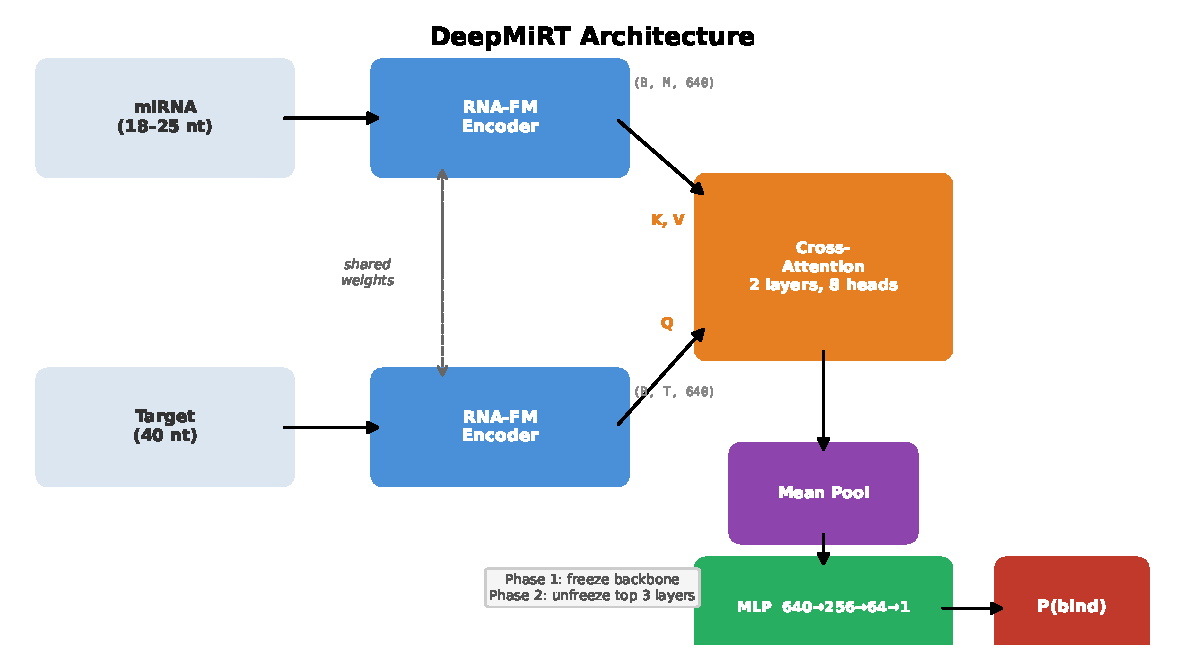
\includegraphics[width=0.85\textwidth]{figures/fig1_architecture.pdf}
\caption{DeepMiRT architecture. A shared RNA-FM encoder produces contextual embeddings for both miRNA and target sequences. Cross-attention (2 layers, 8 heads) enables the target to attend to the miRNA. Masked mean pooling and an MLP head output a binding probability. The RNA-FM backbone is frozen during training; only the cross-attention and classifier head are optimized ($\sim$4M trainable parameters out of 103M total).}
\label{fig:architecture}
\end{figure}

\begin{figure}[!htbp]
\centering
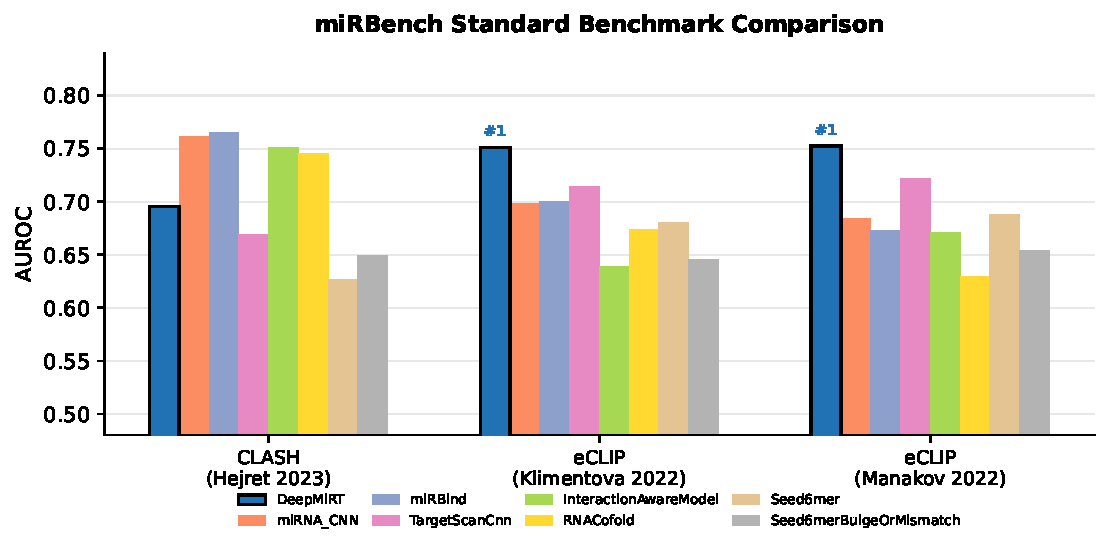
\includegraphics[width=0.85\textwidth]{figures/fig2_benchmark.pdf}
\caption{Benchmark comparison on miRBench test datasets. Grouped bar chart showing AUROC (computed by us using the miRBench framework) for the top 8 methods across three datasets. DeepMiRT (blue, highlighted) ranks first on both eCLIP datasets.}
\label{fig:benchmark}
\end{figure}

\begin{figure}[!htbp]
\centering
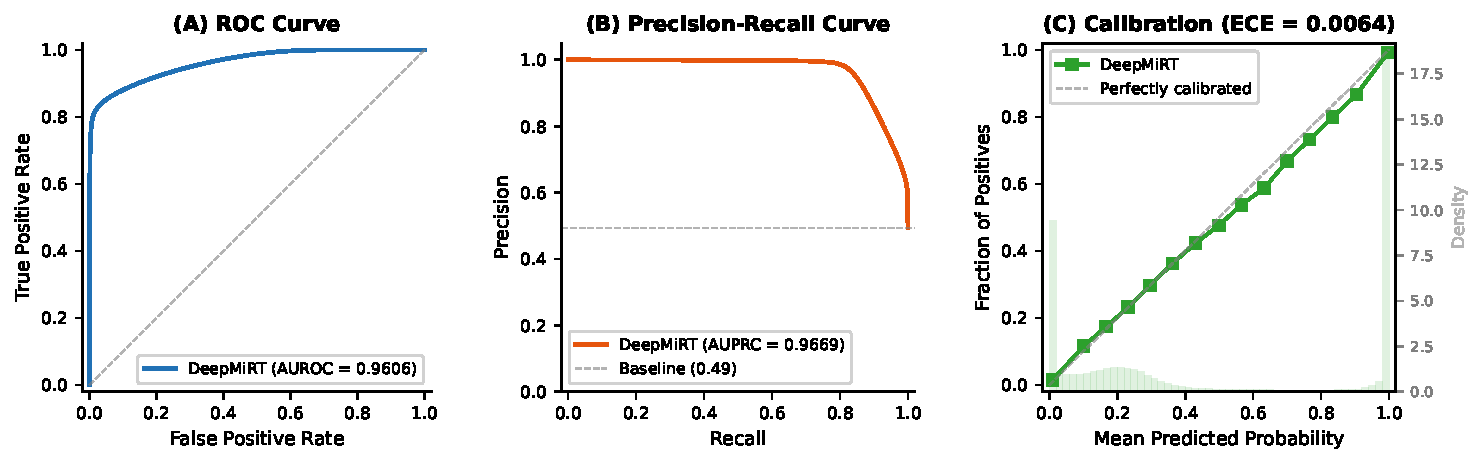
\includegraphics[width=\textwidth]{figures/fig3_performance.pdf}
\caption{Test set performance (813{,}329 samples). (A) ROC curve (AUROC = 0.9606). (B) Precision-recall curve (AUPRC = 0.9669). (C) Calibration reliability diagram (ECE = 0.0064), showing that predicted probabilities closely match observed binding frequencies. The background histogram shows the distribution of predicted probabilities.}
\label{fig:performance}
\end{figure}

% ============================================================
% References
% ============================================================
\bibliography{references}

\end{document}
